\documentclass[12pt,a4paper]{article}

% --- Encoding & Fonts ---
\usepackage[utf8]{inputenc}
\usepackage[T1]{fontenc}
\usepackage{mathpazo}              % Palatino for body text
\usepackage{inconsolata}           % Better monospace font for code
\usepackage[margin=2.5cm]{geometry}

% --- Graphics & Diagrams ---
\usepackage{graphicx}
\usepackage{tikz}
\usetikzlibrary{arrows.meta,positioning,shapes.geometric,calc}

% --- Tables & Lists ---
\usepackage{booktabs}
\usepackage{enumitem}
\usepackage{caption}
\usepackage{float}
\setlist{itemsep=2pt, topsep=4pt}  % Tighter list spacing

% --- Code Listings ---
\usepackage{listings}
\usepackage{xcolor}

\definecolor{codegreen}{rgb}{0.2,0.55,0.2}
\definecolor{codegray}{rgb}{0.45,0.45,0.45}
\definecolor{codepurple}{rgb}{0.5,0.0,0.7}
\definecolor{backcolour}{rgb}{0.97,0.97,0.98}
\definecolor{framerule}{rgb}{0.78,0.78,0.82}
\definecolor{linkblue}{rgb}{0.1,0.3,0.65}
\definecolor{sectionblue}{rgb}{0.12,0.25,0.50}

\lstdefinestyle{gostyle}{
    backgroundcolor=\color{backcolour},
    commentstyle=\itshape\color{codegreen},
    keywordstyle=\bfseries\color{blue!80!black},
    numberstyle=\scriptsize\color{codegray},
    stringstyle=\color{codepurple},
    basicstyle=\ttfamily\small,
    breaklines=true,
    numbers=left,
    numbersep=8pt,
    frame=single,
    framesep=6pt,
    xleftmargin=14pt,
    rulecolor=\color{framerule},
    tabsize=4,
    captionpos=b,
    showstringspaces=false,
    aboveskip=10pt,
    belowskip=8pt,
    abovecaptionskip=6pt
}
\lstset{style=gostyle}

% --- Hyperlinks ---
\usepackage{hyperref}
\hypersetup{
    colorlinks=true,
    linkcolor=linkblue,
    urlcolor=linkblue,
    citecolor=linkblue,
    pdftitle={MetaChat: E2E Encrypted Messaging},
    pdfauthor={Mehdi Talebikhatir, Benyamin Baharizadeh}
}

% --- Section Styling ---
\usepackage{titlesec}
\titleformat{\section}{\Large\bfseries\color{sectionblue}}{\thesection}{1em}{}
\titleformat{\subsection}{\large\bfseries\color{sectionblue!80}}{\thesubsection}{0.8em}{}
\titlespacing*{\section}{0pt}{18pt}{10pt}
\titlespacing*{\subsection}{0pt}{14pt}{6pt}

% --- Math ---
\usepackage{amsmath}
\usepackage{amssymb}

% --- Header / Footer ---
\usepackage{fancyhdr}
\pagestyle{fancy}
\fancyhf{}
\fancyhead[L]{\small\itshape MetaChat -- Secure Messaging}
\fancyhead[R]{\small\itshape University of Messina}
\fancyfoot[C]{\thepage}
\renewcommand{\headrulewidth}{0.4pt}
\renewcommand{\footrulewidth}{0pt}

% --- Caption Styling ---
\captionsetup{font=small, labelfont=bf, skip=6pt}

% --- Paragraph Spacing ---
\setlength{\parskip}{4pt}
\setlength{\parindent}{0pt}

\begin{document}

% --- COVER PAGE ---
\begin{titlepage}
\centering
\vspace*{1cm}
{\Large\textsc{University of Messina}}\\[0.3cm]
{\large Department of Engineering}\\[2cm]
\rule{\linewidth}{0.5mm}\\[0.5cm]
{\LARGE\bfseries MetaChat: End-to-End Encrypted Messaging\\[0.3cm]
Using Extended Triple Diffie-Hellman \&\\Double Ratchet in Go}\\[0.5cm]
\rule{\linewidth}{0.5mm}\\[2cm]
{\large\textbf{Project Report}}\\[2cm]
\begin{tabular}{l l}
\textbf{Authors:} & Mehdi Talebikhatir \quad (ID: 558948) \\
                   & Benyamin Baharizadeh \quad (ID: 560587) \\[1cm]
\textbf{Repository:} & \url{https://github.com/mehditalebi01/metachat} \\[0.5cm]
\textbf{Language:} & Go 1.24 \\
\textbf{Date:} & April 2026 \\
\end{tabular}
\vfill
\end{titlepage}

\tableofcontents
\newpage

% ============================================================
\section{Abstract}
% ============================================================

This report presents MetaChat, a working demonstration of end-to-end encrypted messaging written in Go. The project shows how two users can exchange messages through an untrusted relay server without the server ever seeing the plaintext. We use X25519 elliptic-curve Diffie-Hellman for key exchange, HKDF-SHA256 for key derivation, a Double Ratchet mechanism for forward secrecy, and AES-256-GCM for authenticated encryption. The relay server stores only ciphertext blobs and public keys in Redis, acting as a zero-knowledge intermediary. This report walks through the design, architecture, implementation details, and outputs of the system step by step.

% ============================================================
\section{Introduction}
% ============================================================

\subsection{Background and Motivation}

Messaging applications are part of everyday life. Apps like WhatsApp, Signal, and Telegram handle billions of messages daily. A key concern is: who can read those messages? If the server can read them, a hack or a court order means all conversations are exposed.

End-to-end encryption (E2EE) solves this. With E2EE, messages are encrypted on the sender's device and decrypted only on the receiver's device. The server in between only sees encrypted data that it cannot decrypt.

The Signal Protocol, used by Signal, WhatsApp, and others, is the most widely adopted E2EE protocol. It combines several cryptographic techniques:
\begin{itemize}
    \item \textbf{X3DH (Extended Triple Diffie-Hellman):} For establishing a shared secret between two parties who may not be online at the same time.
    \item \textbf{Double Ratchet:} For deriving new encryption keys for every message, giving forward secrecy.
    \item \textbf{AES-GCM:} For the actual message encryption with integrity checking.
\end{itemize}

\subsection{Project Goal}

The goal of MetaChat is to build a minimal but functional implementation of these ideas in Go. We wanted to understand how the Signal Protocol works at a low level by building it ourselves, using only the Go standard library and \texttt{golang.org/x/crypto} --- no third-party cryptographic frameworks.

The system has three components: a sender (Matteo), a receiver (Benny), and a relay server backed by Redis. The server never sees plaintext.

\subsection{Scope}

This is an educational project. We implement the core cryptographic flow (key exchange, ratchet, encryption) but we do not implement some production features like identity verification, replay protection, or TLS. These are discussed in Section~\ref{sec:discussion}.

% ============================================================
\section{Cryptographic Foundations}
% ============================================================

Before going into the implementation, we briefly explain the cryptographic building blocks.

\subsection{X25519 Diffie-Hellman Key Exchange}

Diffie-Hellman (DH) allows two parties to agree on a shared secret over an insecure channel. X25519 is an elliptic-curve variant using Curve25519. Each party generates a private key (32 random bytes) and computes a public key by multiplying with the curve's base point. When party A computes $X25519(a_{priv}, B_{pub})$ and party B computes $X25519(b_{priv}, A_{pub})$, they get the same shared secret.

\subsection{HKDF-SHA256}

HKDF (HMAC-based Key Derivation Function) takes a shared secret and derives one or more cryptographic keys from it. We use HKDF with SHA-256 and different ``info'' strings (\texttt{"root"}, \texttt{"chain"}, \texttt{"msg"}) to derive separate keys for different purposes.

\subsection{Double Ratchet}

The Double Ratchet algorithm provides forward secrecy. The idea is simple: after deriving a message key, the chain key is advanced (ratcheted) so that old keys cannot be recovered from the current state. Our implementation includes:
\begin{itemize}
    \item A \textbf{root key} derived from the DH shared secret.
    \item A \textbf{chain key} derived from the root key, advanced with each message.
    \item A \textbf{message key} derived from the current chain key.
    \item A \textbf{DH ratchet step} that re-derives the root and chain keys from a new DH exchange.
\end{itemize}

\subsection{AES-256-GCM}

AES-256-GCM is an authenticated encryption scheme. It encrypts the plaintext and produces a tag that allows the receiver to verify that the ciphertext was not tampered with. The 256-bit key comes from the ratchet's message key. A random 12-byte nonce is generated for each encryption.

% ============================================================
\section{System Architecture}
\label{sec:architecture}
% ============================================================

\subsection{High-Level Overview}

The system consists of three independent processes that communicate over HTTP:

\begin{figure}[H]
\centering
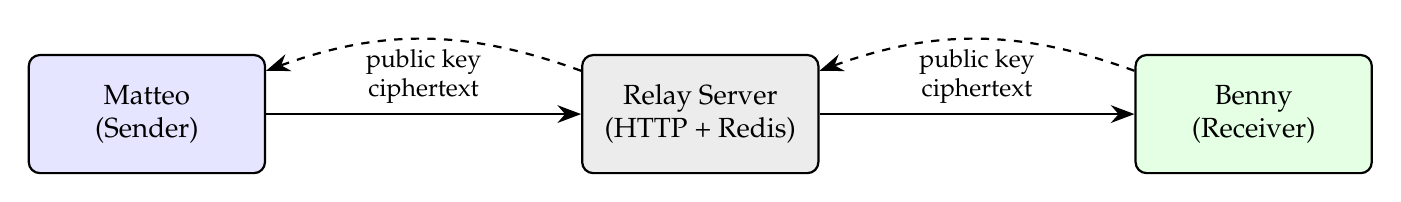
\begin{tikzpicture}[
    node distance=4cm,
    box/.style={rectangle, draw, rounded corners, minimum width=3cm, minimum height=1.5cm, align=center, thick},
    arrow/.style={-{Stealth[length=3mm]}, thick}
]
    \node[box, fill=blue!10] (matteo) {Matteo\\(Sender)};
    \node[box, fill=gray!15, right=of matteo] (server) {Relay Server\\(HTTP + Redis)};
    \node[box, fill=green!10, right=of server] (benny) {Benny\\(Receiver)};

    \draw[arrow] (matteo) -- node[above]{\small ciphertext} (server);
    \draw[arrow] (server) -- node[above]{\small ciphertext} (benny);
    \draw[arrow, dashed] (benny) to[bend right=20] node[below]{\small public key} (server);
    \draw[arrow, dashed] (server) to[bend right=20] node[below]{\small public key} (matteo);
\end{tikzpicture}
\caption{High-level architecture of MetaChat.}
\label{fig:arch}
\end{figure}

\begin{itemize}
    \item \textbf{Benny (Receiver):} Generates an X25519 identity keypair, uploads the public key to the server, and polls for incoming encrypted messages.
    \item \textbf{Matteo (Sender):} Fetches Benny's public key, performs DH key exchange, derives keys via the ratchet, encrypts the message with AES-GCM, and sends the ciphertext to the server.
    \item \textbf{Server:} An HTTP server backed by Redis. It stores public keys and queues encrypted messages. It never performs any decryption.
\end{itemize}

\subsection{Message Sequence}

The complete message exchange follows these steps in order:

\begin{table}[H]
\centering
\small
\begin{tabular}{c l l l}
\toprule
\textbf{Step} & \textbf{From $\rightarrow$ To} & \textbf{Action} & \textbf{Data} \\
\midrule
1 & Benny (local) & Generate X25519 identity keypair & -- \\
2 & Benny $\rightarrow$ Server & Upload public key & \texttt{identity\_key} (32\,B) \\
3 & Matteo $\rightarrow$ Server & Fetch Benny's public key & -- \\
4 & Server $\rightarrow$ Matteo & Return prekey bundle & \texttt{identity\_key} (32\,B) \\
5 & Matteo (local) & DH $\rightarrow$ Ratchet $\rightarrow$ AES-GCM encrypt & -- \\
6 & Matteo $\rightarrow$ Server & Send encrypted payload & \texttt{nonce} + \texttt{ciphertext} \\
7 & Benny $\rightarrow$ Server & Poll mailbox & -- \\
8 & Server $\rightarrow$ Benny & Return encrypted message & \texttt{nonce} + \texttt{ciphertext} \\
9 & Benny (local) & DH $\rightarrow$ Ratchet $\rightarrow$ AES-GCM decrypt & plaintext \\
\bottomrule
\end{tabular}
\caption{Step-by-step message exchange sequence.}
\label{tab:seq}
\end{table}

\vspace{-4pt}

\begin{figure}[H]
\centering
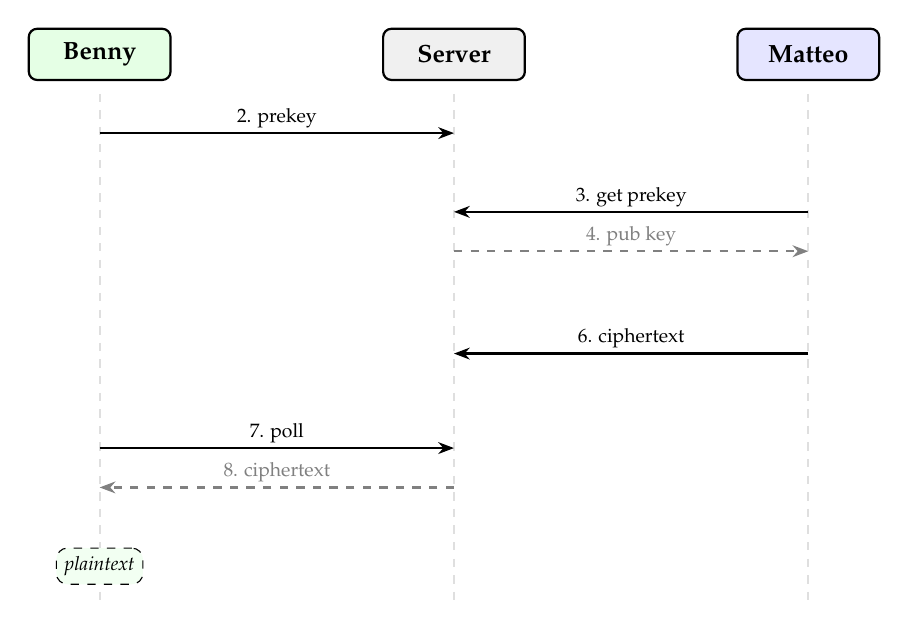
\begin{tikzpicture}[
    box/.style={rectangle, draw, thick, rounded corners=3pt, minimum width=1.8cm, minimum height=0.65cm, font=\small\bfseries},
    arr/.style={-{Stealth[length=2mm]}, thick},
    lbl/.style={font=\scriptsize, fill=white, inner sep=1.5pt}
]
    \node[box, fill=green!10] (B) at (0,0) {Benny};
    \node[box, fill=gray!12]  (S) at (4.5,0) {Server};
    \node[box, fill=blue!10]  (M) at (9,0) {Matteo};

    \draw[thick, gray!25, dashed] (0,-0.5)--(0,-7);
    \draw[thick, gray!25, dashed] (4.5,-0.5)--(4.5,-7);
    \draw[thick, gray!25, dashed] (9,-0.5)--(9,-7);

    \draw[arr] (0,-1.0)   -- node[lbl,above]{2. prekey}          (4.5,-1.0);
    \draw[arr] (9,-2.0)   -- node[lbl,above]{3. get prekey}      (4.5,-2.0);
    \draw[arr,dashed,gray] (4.5,-2.5) -- node[lbl,above]{4. pub key} (9,-2.5);
    \draw[arr] (9,-3.8)   -- node[lbl,above]{6. ciphertext}      (4.5,-3.8);
    \draw[arr] (0,-5.0)   -- node[lbl,above]{7. poll}            (4.5,-5.0);
    \draw[arr,dashed,gray] (4.5,-5.5) -- node[lbl,above]{8. ciphertext} (0,-5.5);
    \node[rectangle, draw, dashed, rounded corners, fill=green!5, font=\scriptsize\itshape, inner sep=3pt] at (0,-6.5) {plaintext};
\end{tikzpicture}
\caption{Simplified sequence diagram of the message exchange.}
\label{fig:seq}
\end{figure}

\subsection{Project Structure}

\begin{table}[H]
\centering
\begin{tabular}{l p{8cm}}
\toprule
\textbf{Path} & \textbf{Description} \\
\midrule
\texttt{server/main.go} & HTTP relay server with Redis backend \\
\texttt{matteo/main.go} & Sender client -- encrypts and sends messages \\
\texttt{benny/main.go} & Receiver client -- polls, decrypts, displays \\
\texttt{internal/crypto/crypto.go} & X25519, HKDF-SHA256, AES-256-GCM functions \\
\texttt{internal/ratchet/ratchet.go} & Double Ratchet key derivation chain \\
\texttt{go.mod} & Module definition and dependencies \\
\bottomrule
\end{tabular}
\caption{Project file structure.}
\end{table}

\subsection{Server API}

The relay server exposes four HTTP endpoints:

\begin{table}[H]
\centering
\begin{tabular}{l l p{6cm}}
\toprule
\textbf{Method} & \textbf{Endpoint} & \textbf{Description} \\
\midrule
POST & \texttt{/upload\_prekey?user=X} & Upload user's public key \\
GET  & \texttt{/prekey?user=X} & Fetch a user's public key \\
POST & \texttt{/send\_secure?to=X} & Queue encrypted message \\
GET  & \texttt{/fetch\_secure?user=X} & Pop next message from mailbox \\
\bottomrule
\end{tabular}
\caption{Server API endpoints.}
\end{table}

Data is stored in Redis under two key patterns: \texttt{prekey:<user>} (string, JSON public key bundle) and \texttt{secure\_mailbox:<user>} (list, queue of encrypted messages).

\subsection{Dependencies}

The project uses minimal external dependencies, relying mostly on the Go standard library:

\begin{table}[H]
\centering
\begin{tabular}{l l p{6.5cm}}
\toprule
\textbf{Module} & \textbf{Version} & \textbf{Purpose} \\
\midrule
\texttt{golang.org/x/crypto} & v0.48.0 & X25519 (\texttt{curve25519}), HKDF-SHA256 (\texttt{hkdf}) \\
\texttt{github.com/redis/go-redis/v9} & v9.18.0 & Redis client for key storage and message queuing \\
\texttt{crypto/aes}, \texttt{crypto/cipher} & stdlib & AES-256-GCM authenticated encryption \\
\texttt{crypto/rand} & stdlib & Cryptographically secure random bytes \\
\texttt{net/http} & stdlib & HTTP server and client \\
\bottomrule
\end{tabular}
\caption{Project dependencies and their roles.}
\end{table}

\subsection{Message Payload Structure}

The encrypted message sent over the wire is a JSON object with four fields. Below is an example of what the server sees (all binary fields are Base64-encoded by Go's JSON marshaler):

\begin{lstlisting}[language={}, caption={Example SecureMessage JSON payload (server's view).}, numbers=none]
{
  "from_identity": "a3RmZ2hqa2xhc2RmZ2hqa2xh...",
  "ephemeral_key": "a3RmZ2hqa2xhc2RmZ2hqa2xh...",
  "nonce":         "dGhpcyBpcyBhIG5vbmNl",
  "ciphertext":    "Y2lwaGVydGV4dCBibG9iIGhlcmU..."
}
\end{lstlisting}

\begin{table}[H]
\centering
\begin{tabular}{l l p{5.8cm}}
\toprule
\textbf{Field} & \textbf{Size} & \textbf{Description} \\
\midrule
\texttt{from\_identity} & 32 bytes & Sender's public key (for identification) \\
\texttt{ephemeral\_key} & 32 bytes & Sender's ephemeral X25519 public key (used by receiver for DH) \\
\texttt{nonce} & 12 bytes & Random AES-GCM nonce \\
\texttt{ciphertext} & variable & AES-GCM sealed message (ciphertext + 16-byte auth tag) \\
\bottomrule
\end{tabular}
\caption{Fields of the SecureMessage payload.}
\end{table}

The server stores and forwards this JSON blob without interpreting any of the fields. It has no access to the shared secret or message key needed to decrypt \texttt{ciphertext}.

% ============================================================
\section{Implementation Details}
\label{sec:implementation}
% ============================================================

This section walks through the actual Go code and explains how each component works.

\subsection{Cryptographic Module (\texttt{internal/crypto/crypto.go})}

This module provides four core functions:

\begin{lstlisting}[language=Go, caption={Crypto module -- key generation, DH, and HKDF.}]
package crypto

import (
    "crypto/aes"
    "crypto/cipher"
    "crypto/rand"
    "crypto/sha256"
    "io"
    "golang.org/x/crypto/hkdf"
    "golang.org/x/crypto/curve25519"
)

func GenerateKeyPair() (priv, pub []byte) {
    priv = make([]byte, 32)
    rand.Read(priv)
    pub, _ = curve25519.X25519(priv, curve25519.Basepoint)
    return
}

func DH(priv, pub []byte) []byte {
    shared, _ := curve25519.X25519(priv, pub)
    return shared
}

func HKDF(secret []byte, info string) []byte {
    h := hkdf.New(sha256.New, secret, nil, []byte(info))
    out := make([]byte, 32)
    io.ReadFull(h, out)
    return out
}
\end{lstlisting}

\begin{lstlisting}[language=Go, caption={Crypto module -- AES-256-GCM encrypt/decrypt.}]
func Encrypt(key, plaintext []byte) (nonce, ciphertext []byte) {
    block, _ := aes.NewCipher(key)
    gcm, _ := cipher.NewGCM(block)
    nonce = make([]byte, gcm.NonceSize())
    rand.Read(nonce)
    ciphertext = gcm.Seal(nil, nonce, plaintext, nil)
    return
}

func Decrypt(key, nonce, ciphertext []byte) []byte {
    block, _ := aes.NewCipher(key)
    gcm, _ := cipher.NewGCM(block)
    plaintext, _ := gcm.Open(nil, nonce, ciphertext, nil)
    return plaintext
}
\end{lstlisting}

\textbf{How it works:}
\begin{enumerate}
    \item \texttt{GenerateKeyPair()} fills 32 bytes from the OS random source and multiplies by the Curve25519 base point to get the public key.
    \item \texttt{DH()} multiplies the private key with the other party's public key to get a shared secret.
    \item \texttt{HKDF()} derives a 32-byte key deterministically from a secret and an info label.
    \item \texttt{Encrypt()} creates an AES-256 cipher in GCM mode, generates a random 12-byte nonce, and seals the plaintext.
    \item \texttt{Decrypt()} reverses the process using the same key and nonce.
\end{enumerate}

\subsection{Ratchet Module (\texttt{internal/ratchet/ratchet.go})}

\begin{lstlisting}[language=Go, caption={Double Ratchet implementation.}]
package ratchet

import "metachat/internal/crypto"

type Ratchet struct {
    RootKey   []byte
    ChainKey  []byte
    DHPriv    []byte
    DHPub     []byte
    RemotePub []byte
}

func NewRatchet(sharedSecret, remotePub []byte) *Ratchet {
    priv, pub := crypto.GenerateKeyPair()
    root := crypto.HKDF(sharedSecret, "root")
    chain := crypto.HKDF(root, "chain")
    return &Ratchet{
        RootKey: root, ChainKey: chain,
        DHPriv: priv, DHPub: pub, RemotePub: remotePub,
    }
}

func (r *Ratchet) RatchetStep() {
    dhOut := crypto.DH(r.DHPriv, r.RemotePub)
    r.RootKey = crypto.HKDF(dhOut, "root")
    r.ChainKey = crypto.HKDF(r.RootKey, "chain")
    r.DHPriv, r.DHPub = crypto.GenerateKeyPair()
}

func (r *Ratchet) NextMessageKey() []byte {
    r.ChainKey = crypto.HKDF(r.ChainKey, "chain-step")
    return crypto.HKDF(r.ChainKey, "msg")
}
\end{lstlisting}

The \texttt{Ratchet} struct holds the current state. Each call to \texttt{NextMessageKey()} advances the chain key forward and derives a message key. The old chain key is overwritten, so previous message keys cannot be recovered -- this is forward secrecy.

\subsection{Key Derivation Flow}

\begin{figure}[H]
\centering
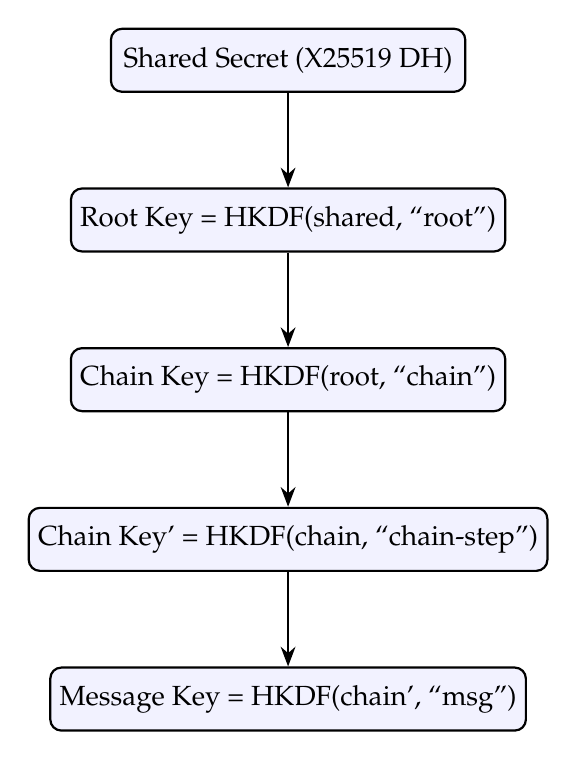
\begin{tikzpicture}[
    node distance=1.2cm,
    block/.style={rectangle, draw, rounded corners, minimum width=4.5cm, minimum height=0.8cm, align=center, thick, fill=blue!5},
    arrow/.style={-{Stealth[length=2.5mm]}, thick}
]
    \node[block] (shared) {Shared Secret (X25519 DH)};
    \node[block, below=of shared] (root) {Root Key = HKDF(shared, ``root'')};
    \node[block, below=of root] (chain) {Chain Key = HKDF(root, ``chain'')};
    \node[block, below=of chain] (step) {Chain Key' = HKDF(chain, ``chain-step'')};
    \node[block, below=of step] (msg) {Message Key = HKDF(chain', ``msg'')};
    \draw[arrow] (shared) -- (root);
    \draw[arrow] (root) -- (chain);
    \draw[arrow] (chain) -- (step);
    \draw[arrow] (step) -- (msg);
\end{tikzpicture}
\caption{Key derivation chain from shared secret to message key.}
\label{fig:kdf}
\end{figure}

\subsection{Sender: Matteo (\texttt{matteo/main.go})}

\begin{lstlisting}[language=Go, caption={Core sending logic (simplified).}]
// Fetch Benny's prekey from server
resp, _ := http.Get("http://localhost:8080/prekey?user=benny")
var bundle PrekeyBundle
json.NewDecoder(resp.Body).Decode(&bundle)

// Generate ephemeral keypair and compute shared secret
matteoPriv, matteoPub := crypto.GenerateKeyPair()
shared := crypto.DH(matteoPriv, bundle.IdentityKey)

// Initialize ratchet and derive message key
r := ratchet.NewRatchet(shared, bundle.IdentityKey)
msgKey := r.NextMessageKey()

// Encrypt and send
nonce, ciphertext := crypto.Encrypt(msgKey, []byte(message))
msg := SecureMessage{
    FromIdentity: matteoPub, EphemeralKey: matteoPub,
    Nonce: nonce, Ciphertext: ciphertext,
}
data, _ := json.Marshal(msg)
http.Post("http://localhost:8080/send_secure?to=benny",
    "application/json", bytes.NewBuffer(data))
\end{lstlisting}

\subsection{Receiver: Benny (\texttt{benny/main.go})}

\begin{lstlisting}[language=Go, caption={Core receiving logic (simplified).}]
// Generate identity and upload public key
bennyPriv, bennyPub := crypto.GenerateKeyPair()
bundle := PrekeyBundle{IdentityKey: bennyPub}
data, _ := json.Marshal(bundle)
http.Post("http://localhost:8080/upload_prekey?user=benny",
    "application/json", bytes.NewBuffer(data))

// Poll for messages
for {
    resp, _ := http.Get(
        "http://localhost:8080/fetch_secure?user=benny")
    var msg SecureMessage
    json.NewDecoder(resp.Body).Decode(&msg)
    if len(msg.Ciphertext) == 0 {
        time.Sleep(300 * time.Millisecond)
        continue
    }
    shared := crypto.DH(bennyPriv, msg.EphemeralKey)
    r := ratchet.NewRatchet(shared, msg.EphemeralKey)
    msgKey := r.NextMessageKey()
    plaintext := crypto.Decrypt(msgKey, msg.Nonce,
        msg.Ciphertext)
    fmt.Println("[BENNY] Received:", string(plaintext))
    break
}
\end{lstlisting}

Both sides compute the \textit{same} shared secret through DH, so they derive the same message key.

\subsection{Server (\texttt{server/main.go})}

\begin{lstlisting}[language=Go, caption={Server -- message relay handlers.}]
func sendSecure(w http.ResponseWriter, r *http.Request) {
    to := r.URL.Query().Get("to")
    var msg SecureMessage
    json.NewDecoder(r.Body).Decode(&msg)
    data, _ := json.Marshal(msg)
    rdb.LPush(ctx, "secure_mailbox:"+to, data)
    w.Write([]byte("OK"))
}

func fetchSecure(w http.ResponseWriter, r *http.Request) {
    user := r.URL.Query().Get("user")
    val, err := rdb.RPop(ctx, "secure_mailbox:"+user).Result()
    if err == redis.Nil {
        w.Write([]byte("{}"))
        return
    }
    w.Write([]byte(val))
}
\end{lstlisting}

The server \textbf{never} calls any decryption function. It only stores and forwards opaque ciphertext blobs.

% ============================================================
\section{Running the System: Step-by-Step}
\label{sec:running}
% ============================================================

The system requires three terminals:

\subsection{Step 1: Start Redis and the Server}
\begin{lstlisting}[language=bash, caption={Starting the relay server.}]
$ go run ./server
[SERVER] Running on :8080 (Redis: localhost:6379)
\end{lstlisting}

\subsection{Step 2: Start Benny (Receiver)}
\begin{lstlisting}[language=bash, caption={Benny starts and uploads his public key.}]
$ go run ./benny
[BENNY] Generating Benny X25519 identity keypair...
[BENNY] Uploading Benny public key to server
        (stored in Redis as prekey:benny)...
[BENNY] Benny ready. Polling mailbox from server
        (secure_mailbox:benny in Redis)...
\end{lstlisting}

\subsection{Step 3: Send a Message as Matteo}
\begin{lstlisting}[language=bash, caption={Matteo encrypts and sends a message.}]
$ go run ./matteo Hello Benny, this is a secret message!
[MATTEO] Fetching Benny prekey from server...
[MATTEO] Benny prekey received.
[MATTEO] Generating Matteo ephemeral X25519 keypair...
[MATTEO] Computing shared secret (X25519 DH)...
[MATTEO] Initializing ratchet and deriving message key...
[MATTEO] Encrypting message with AES-GCM...
[MATTEO] Sending encrypted message to server...
[MATTEO] Done. Message sent.
\end{lstlisting}

\subsection{Step 4: Benny Receives and Decrypts}
\begin{lstlisting}[language=bash, caption={Benny decrypts the message.}]
[BENNY] Received encrypted message.
        Deriving shared secret (X25519 DH)...
[BENNY] Initializing ratchet and deriving message key...
[BENNY] Decrypting with AES-GCM...
[BENNY] Benny received: Hello Benny, this is a secret message!
\end{lstlisting}

The message went through the server encrypted and was only decrypted on Benny's side.

% ============================================================
\section{Results and Discussion}
\label{sec:discussion}
% ============================================================

\subsection{What Works}
The implementation successfully demonstrates:
\begin{itemize}
    \item X25519 key exchange between two parties through an untrusted server.
    \item Key derivation using HKDF with a ratchet chain that provides forward secrecy.
    \item AES-256-GCM authenticated encryption preventing the server from reading messages.
    \item Asynchronous message delivery through Redis mailboxes.
\end{itemize}

\subsection{Security Analysis}

\begin{table}[H]
\centering
\begin{tabular}{l c p{5.5cm}}
\toprule
\textbf{Property} & \textbf{Status} & \textbf{Notes} \\
\midrule
Authenticated encryption & \checkmark & AES-256-GCM \\
Key exchange & \checkmark & X25519 ECDH \\
Forward secrecy (chain) & \checkmark & Chain key ratcheting \\
Zero-knowledge server & \checkmark & Server sees only ciphertext \\
Identity verification & $\times$ & No certificate pinning \\
Replay protection & $\times$ & No message counters \\
Transport security & $\times$ & HTTP, not TLS \\
Multi-message sessions & $\times$ & Benny exits after one message \\
\bottomrule
\end{tabular}
\caption{Security properties of the implementation.}
\end{table}

\subsection{Limitations and Future Work}
For a production system, the following would need to be added:
\begin{itemize}
    \item TLS for all client-server communication.
    \item Identity verification through safety numbers or QR codes.
    \item Message ordering with sequence numbers and replay detection.
    \item Persistent key storage so keys survive restarts.
    \item Full Double Ratchet with header encryption.
    \item Multi-device support and group messaging.
\end{itemize}

% ============================================================
\section{Appendix: Modern Messengers and E2EE}
\label{sec:appendix}
% ============================================================

End-to-end encryption has become standard in modern messaging. Below is a comparison:

\begin{table}[H]
\centering
\begin{tabular}{l c l l}
\toprule
\textbf{App} & \textbf{E2EE Default} & \textbf{Protocol} & \textbf{Notes} \\
\midrule
Signal     & Yes & Signal Protocol & Open source, gold standard \\
WhatsApp   & Yes & Signal Protocol & Uses Signal's library \\
Telegram   & No  & MTProto & E2EE only in ``Secret Chats'' \\
iMessage   & Yes & Custom (Apple) & Closed source \\
Messenger  & Yes & Signal Protocol & Default since Dec 2023 \\
\bottomrule
\end{tabular}
\caption{E2EE in popular messaging applications.}
\end{table}

The Signal Protocol, which MetaChat is inspired by, combines X3DH for initial key exchange and Double Ratchet for ongoing encryption, providing both forward secrecy and future secrecy. Our project implements a simplified version of this pipeline, demonstrating the core ideas in a readable way.

% ============================================================
\section{Testing and Verification}
\label{sec:testing}
% ============================================================

We verified the correctness of the system through the following methods:

\subsection{Functional Testing}

The primary test was running the full message exchange pipeline end-to-end:
\begin{enumerate}
    \item Start Redis and verify connectivity (\texttt{redis-cli ping} returns \texttt{PONG}).
    \item Start the server and confirm it binds to port 8080.
    \item Start Benny and verify that the server logs the prekey storage (\texttt{prekey:benny} key appears in Redis).
    \item Send a message as Matteo with a known plaintext string.
    \item Verify that Benny's terminal output shows the exact same plaintext, confirming that key exchange, ratchet derivation, encryption, and decryption all produce consistent results.
\end{enumerate}

We repeated this test with different message lengths (short strings, paragraphs, special characters including Unicode) to confirm that AES-GCM handles variable-length input correctly.

\subsection{Negative Testing}

We also tested failure scenarios:
\begin{itemize}
    \item \textbf{Wrong key:} Manually modifying the ephemeral key in a queued Redis message causes Benny to derive a different shared secret, and \texttt{gcm.Open()} returns \texttt{nil} (authentication failure). This confirms that AES-GCM rejects tampered ciphertext.
    \item \textbf{Server down:} If the server is not running, both Matteo and Benny print clear error messages and exit gracefully.
    \item \textbf{No prekey:} If Matteo runs before Benny uploads his key, the server returns HTTP 404 and Matteo exits with an instruction to start Benny first.
\end{itemize}

\subsection{Key Verification}

We added temporary debug prints during development to confirm that the shared secret computed by Matteo (\texttt{DH(matteo\_priv, benny\_pub)}) and Benny (\texttt{DH(benny\_priv, matteo\_ephemeral)}) were byte-identical. Both produced the same 32-byte value, confirming the correctness of the X25519 key exchange.

% ============================================================
\section{Conclusion}
% ============================================================

In this project, we built MetaChat, an end-to-end encrypted messaging system in Go. The system demonstrates how modern secure messaging works at a fundamental level: X25519 key exchange, HKDF key derivation, Double Ratchet for forward secrecy, and AES-256-GCM for authenticated encryption.

The relay server acts as a zero-knowledge intermediary --- it stores and forwards ciphertext without ever accessing plaintext. This mirrors the design philosophy of production messengers like Signal.

While the implementation is educational and lacks some production features (TLS, identity verification, replay protection), it provides a clear, working demonstration of the cryptographic principles that protect billions of messages every day.

\begin{thebibliography}{9}
\bibitem{signal} Marlinspike, M. and Perrin, T. ``The X3DH Key Agreement Protocol,'' Signal Foundation, 2016.
\bibitem{doubleratchet} Perrin, T. and Marlinspike, M. ``The Double Ratchet Algorithm,'' Signal Foundation, 2016.
\bibitem{curve25519} Bernstein, D.J. ``Curve25519: New Diffie-Hellman Speed Records,'' PKC 2006.
\bibitem{aesgcm} Dworkin, M. ``Recommendation for Block Cipher Modes of Operation: Galois/Counter Mode,'' NIST SP 800-38D, 2007.
\bibitem{hkdf} Krawczyk, H. and Eronen, P. ``HMAC-based Extract-and-Expand Key Derivation Function (HKDF),'' RFC 5869, 2010.
\end{thebibliography}

\end{document}
